% Expert Systems with Applications -- DysLex-Probe (journal version)
% Build with XeLaTeX (Bangla glyphs need fontspec): xelatex main.tex (run 2-3x)
% NOTE: no em-dashes anywhere in rendered text; use -- (en-dash) or rewrite.
\documentclass[preprint,12pt]{elsarticle}

\usepackage{fontspec}
\setmainfont{TeX Gyre Termes}
\newfontfamily\banglafont[Script=Bengali]{Noto Serif Bengali}
\newcommand{\bn}[1]{{\banglafont #1}}

\usepackage{amsmath,amssymb}
\usepackage{booktabs}
\usepackage{array}
\usepackage{multirow}
\usepackage{graphicx}
\graphicspath{{figs/}}
\usepackage{float}
\usepackage{url}
\usepackage[hidelinks]{hyperref}

% Float placement: keep figures near their references instead of flushing them to the end.
\renewcommand{\topfraction}{0.9}
\renewcommand{\bottomfraction}{0.85}
\renewcommand{\textfraction}{0.08}
\renewcommand{\floatpagefraction}{0.75}
\setcounter{topnumber}{3}
\setcounter{totalnumber}{5}

% Small padding between a (top) table caption and the table body.
\setlength{\belowcaptionskip}{6pt}

\journal{Expert Systems with Applications}

% ---------------------------------------------------------------------------
% HIGHLIGHTS (for the separate Elsevier highlights file):
%  - Surface controls invalidate three of four standard phonological probing tasks.
%  - Byte-level ByT5 transfers 0.32 F1 higher than subword mT5 (95% CI [0.15,0.49]).
%  - Tokenization, not the encoder-decoder objective, drives cross-lingual collapse.
%  - Subword encoders localize the lexical signal; byte and decoder models distribute it.
%  - LLM features beat a surface baseline on cross-lingual lexical, not graded, screening tasks.
% ---------------------------------------------------------------------------

\begin{document}

\begin{frontmatter}

\title{Surface-controlled cross-lingual probing of multilingual language models for low-resource Bangla dyslexia screening: the roles of tokenization, transfer and localization}

\author[bracu]{Ayesha Siddika\corref{cor1}}
\author[bracu]{Nazmoon Nahar Aka}
\author[bracu]{Mashrafi Rahman}
\author[bracu]{Hasan Mohammad Sayem}
\author[bracu]{Md.\ Tanzim Reza}
\author[bracu]{Farig Yousuf Sadeque}

\affiliation[bracu]{organization={Department of Computer Science and Engineering, BRAC University},
                    city={Dhaka},
                    country={Bangladesh}}

\cortext[cor1]{Corresponding author}

\begin{abstract}
Dyslexia screening in low-resource languages is constrained by the scarcity of expert clinicians, validated test batteries and labelled corpora. Multilingual large language models (LLMs) are an attractive expert-systems substrate, but it is not known which architectures carry lexical information that transfers from a high-resource source (English) to a low-resource target (Bangla), where that information resides, or how tokenization affects it. We probe five publicly released multilingual LLMs spanning the dominant pretraining recipes -- XLM-RoBERTa large, Llama~3.1 8B, BLOOM 7B1, mT5 XL and ByT5 XL -- with frozen per-layer linear probes on a curated 440-item English/Bangla stimulus set, reporting bootstrap confidence intervals throughout. Under first-character, character-statistic and length-matching controls, three of four standard phonological probing tasks fail; only real-versus-pseudoword discrimination survives. On zero-shot Bangla transfer, BLOOM and ByT5 reach 0.92 F1 (95\% CI [0.84, 0.98]) and XLM-R 0.86, while Llama (0.63) and mT5 (0.60) collapse to the surface baseline. Because ByT5 and mT5 share architecture and pretraining objective and differ chiefly in tokenization, ByT5's 0.32 F1 advantage (95\% CI [0.15, 0.49]) identifies tokenization, not the encoder-decoder objective, as the cause of mT5's collapse. Causal ablation reveals a double dissociation: subword encoders localize the transferable signal, whereas byte-level and decoder models distribute it. Finally, a downstream cross-lingual classifier (train on English, test on Bangla) transfers categorical lexical structure above a surface baseline, most strongly under byte-level tokenization, but not abstract graded item properties. Pretraining coverage, objective and tokenization, not parameter scale, determine cross-lingual lexical transfer.
\end{abstract}

\begin{keyword}
multilingual language models \sep cross-lingual transfer \sep probing classifiers \sep dyslexia screening \sep low-resource Bangla NLP \sep tokenization \sep mechanistic interpretability \sep bootstrap confidence intervals
\end{keyword}

\end{frontmatter}

% ===========================================================================
\section{Introduction}
\label{sec:intro}
Developmental dyslexia is a specific learning difficulty that impairs accurate and fluent word reading, decoding and spelling despite adequate intelligence, schooling and sensory function \cite{snowling2020dyslexia,peterson2012developmental}. Estimated prevalence ranges from five to twelve percent of school-age children depending on language and writing system \cite{ziegler2005reading,wagner2020prevalence}, and the dominant cognitive account is the \emph{phonological deficit hypothesis}: dyslexic readers are weaker at representing, retrieving and manipulating speech sounds, which slows grapheme-to-phoneme mapping during reading acquisition \cite{snowling2020dyslexia,goswami2011temporal}.

Clinical identification depends on standardised, language-specific test batteries such as CTOPP-2 \cite{wagner2013ctopp}, which require trained psychometricians and do not exist for most of the world's languages. Bangla, with more than 270 million speakers, has no widely deployed normative dyslexia screener and no consensus diagnostic battery \cite{nag2014dyslexia,nag2017indian,badsha2024mall}; suspected cases are identified late or not at all. The absence of such norms is itself a barrier to identification and a primary motivation for this work.

In parallel, multilingual LLMs have crossed a capability threshold at which their hidden representations encode rich, transferable linguistic structure across the languages in their pretraining mix \cite{conneau2020xlmr,scao2022bloom,xue2021mt5}. The same models that drive translation and dialogue are accumulating, as a by-product, the lexical and sub-lexical structure that clinical screening tools probe explicitly. If that structure transfers from a resource-rich language (English, where validated probes and labels exist) to a low-resource language (Bangla, where they do not), a single multilingual model could anchor a family of expert screening prototypes across many languages at once. A genuine phonological representation should generalise across orthographic depth; surface statistics should not.

Three obstacles stand between this promise and a usable expert system. First, much prior probing work uses \emph{unmatched} stimuli, leaving surface confounds such as character length, byte length and first-character identity uncontrolled; a probe that appears to ``recover voicing'' may simply be reading the first character of the word. Second, results are typically reported as point estimates without confidence intervals, so it is unclear which differences are real. Third, the role of the \emph{tokenizer} -- how a model segments text into units before it ever forms a representation -- has not been isolated for cross-lingual clinical probing, even though English and Bangla use disjoint scripts and a subword vocabulary trained largely on Latin script may fragment Bangla very differently from a byte-level model.

This paper addresses all three. Building on a four-model study, we add a fifth model, ByT5, expressly to turn tokenization into a controlled variable, and we re-analyse every headline number with bootstrap confidence intervals. Concretely, we investigate five research questions.
\begin{enumerate}
\item[\textbf{RQ1}] \textbf{(surface validity).} Which standard phonological probing tasks survive first-character, character-statistic and length-matching controls, and therefore reflect phonology rather than surface form?
\item[\textbf{RQ2}] \textbf{(cross-lingual transfer).} Across the canonical pretraining recipes, which models achieve genuine zero-shot English-to-Bangla lexical transfer above the surface baseline, and is transfer driven by parameter scale or by language coverage and pretraining objective?
\item[\textbf{RQ3}] \textbf{(tokenization).} Holding architecture and pretraining objective fixed, does subword-versus-byte tokenization determine whether cross-lingual lexical structure transfers and how it is organised?
\item[\textbf{RQ4}] \textbf{(mechanism and localization).} Is the transferable signal causally localized to a small set of hidden units or distributed across the representation, and does this organisation dissociate by architecture and tokenization?
\item[\textbf{RQ5}] \textbf{(application and model selection).} Does the transferable structure support a downstream cross-lingual screening-property classifier above a surface baseline, and what principled model-selection recommendation follows for low-resource Bangla screening?
\end{enumerate}
These questions translate into four contributions.
\begin{enumerate}
\item \textbf{Methodological.} Under first-character, character-statistic and length-matching controls, three of four standard phonological probing tasks are shown to measure surface artefacts rather than phonology. Surface-matched stimuli and native-verified labels, reported with confidence intervals, are the minimum standard for cross-lingual clinical probing.
\item \textbf{Comparative.} Across five models spanning the canonical pretraining recipes, only multilingual models with adequate Bangla coverage achieve genuine cross-lingual lexical transfer; a 0.56B multilingual encoder beats an 8B English-heavy decoder, so coverage and objective dominate scale.
\item \textbf{Tokenization.} A controlled comparison of two encoder-decoders that share architecture and pretraining objective but differ in tokenization (subword mT5 versus byte-level ByT5) shows that byte-level tokenization changes both \emph{whether} the signal transfers (collapse becomes best-in-class) and \emph{how} it is stored (localized becomes distributed). Tokenization, not the objective, drives mT5's cross-lingual collapse.
\item \textbf{Applied.} A downstream cross-lingual screening-property classifier, trained only on English and evaluated on Bangla against a surface baseline, delimits exactly where the transferable signal lies: in categorical, lexical distinctions (strongest under byte-level tokenization), not in abstract graded item properties. This bounds the honest scope of an LLM-based screening tool.
\end{enumerate}

% ===========================================================================
\section{Background and related work}
\label{sec:related}
\subsection{Dyslexia and the phonological deficit}
The phonological deficit hypothesis holds that the core impairment in dyslexia is in the phonological component of language \cite{snowling2020dyslexia,goswami2011temporal}. Behaviourally, the strongest single marker is impaired \emph{pseudoword reading} \cite{rack1992nonword}: because a pseudoword has no lexical entry, it can only be read by phonological decoding, isolating exactly the skill that breaks down in dyslexia. This motivates a probing design centred on real-versus-pseudoword discrimination and on sound-contrast (minimal-pair) items, and it is the reason the surviving task in our study is the one most directly tied to the clinical marker.

\subsection{Orthographic depth and Bangla}
Orthographic depth -- how directly spelling maps to sound -- predicts cross-language differences in reading acquisition and dyslexia manifestation \cite{ziegler2005reading}. English is orthographically opaque; Bangla is intermediate, with a largely regular consonant inventory but heavy use of conjunct characters (\textit{yuktoborno}) and vowel diacritics (\textit{matra}) that do not transparently decompose. This makes the English-to-Bangla direction a natural cross-lingual testbed: a representation that survives the change of script and depth is encoding structure rather than surface form. The Bangla difficulty patterns documented by Badsha \cite{badsha2024mall} for dyslexic Bangla-speaking children -- voiced/unvoiced confusions, aspiration, conjuncts and multisyllabic load -- ground our Bangla stimulus design.

\subsection{Multilingual LLMs, pretraining recipes and tokenization}
Modern multilingual LLMs, all built on the Transformer architecture \cite{vaswani2017attention}, differ along three axes that this study isolates: pretraining objective, language coverage and tokenization. XLM-RoBERTa \cite{conneau2020xlmr} is a multilingual masked encoder in the BERT family \cite{devlin2019bert}; BLOOM \cite{scao2022bloom} and Llama~3.1 \cite{dubey2024llama3} are causal decoders differing chiefly in coverage (BLOOM is explicitly multilingual, Llama is English-heavy) and both segment text with byte-pair encoding \cite{sennrich2016bpe}; mT5 \cite{xue2021mt5}, the multilingual extension of T5 \cite{raffel2020t5}, is a span-corruption encoder-decoder with a SentencePiece \cite{kudo2018sentencepiece} subword vocabulary; and ByT5 \cite{xue2022byt5} is the byte-level counterpart of mT5, trained on the same corpus with the same objective but operating directly on UTF-8 bytes with no subword vocabulary. Multilingual encoders exhibit emergent cross-lingual structure \cite{pires2019mbert,wu2020emerging,artetxe2020cross}, but coverage is uneven, and the tokenizer strongly shapes how a script is represented \cite{rust2021tokenizer}: a subword vocabulary trained mostly on Latin script fragments Bangla differently from a byte-level model that shares a single 256-symbol alphabet across all scripts. Whether tokenization helps or harms cross-lingual clinical transfer has, to our knowledge, not been isolated.

\subsection{Probing and interpretability}
Linear probing reads target properties from frozen representations with low-capacity classifiers, so success implies the property is linearly available rather than learned by the probe \cite{alain2017probes,conneau2018probing,hewitt2019structural,belinkov2022probing}. The central methodological risk is that probes succeed on confounds rather than the intended property \cite{belinkov2022probing,pimentel2020information}; control baselines and control tasks are therefore essential \cite{hewitt2019control}. Beyond decoding, causal interventions (ablating units and measuring the downstream effect) \cite{vig2020causal,meng2022rome} test whether information is merely decodable or causally used, and Representational Similarity Analysis (RSA) \cite{kriegeskorte2008rsa} compares representational geometry without training any probe. We add bootstrap confidence intervals \cite{efron1994bootstrap} to every headline comparison so that the surviving effects are shown to be statistically, not just numerically, real.

\subsection{Automated dyslexia screening}
Prior computational approaches to dyslexia screening have largely relied on task-specific behavioural signals: supervised models over handwriting samples \cite{spoon2019handwriting}, eye-tracking during reading \cite{benfatto2016eyetracking}, gameplay telemetry \cite{rello2020gamified}, or audio of oral reading \cite{tas2023audio}, typically trained per language on labelled child data. Such pipelines are accurate where data exist but do not transfer to languages without labelled corpora, which is the situation for Bangla. Our approach is complementary and upstream: rather than training a screener, we ask whether the representations of an already-pretrained multilingual model contain the phonological and lexical structure that such a screener would need, and whether that structure transfers across languages. A positive answer identifies a substrate on which a downstream, clinician-supervised screener can later be built without per-language pretraining.

\subsection{Research gap}
We are not aware of prior work that compares the dominant multilingual pretraining recipes on the same surface-controlled cross-lingual lexical task, with the same stimuli and metrics, isolates the tokenizer as a controlled variable, reports confidence intervals, and then localises the signal causally. This study closes that gap and frames it around a concrete low-resource expert-system application.

% ===========================================================================
\section{Stimulus dataset}
\label{sec:data}
\subsection{Design principles}
The dataset is a single 440-item CSV (220 English + 220 Bangla, 18 metadata columns), identical across all five model runs so that any difference is attributable to the models. It is perfectly balanced by language and by category within language, the categories map onto documented dyslexia error types, and the rich metadata exists specifically to support confound control.

\subsection{Categories and counts}
The dataset contains seven phonological task categories (200 items per language) plus a 40-item cross-lingual concept-matching set used for RSA (Table~\ref{tab:data}). Minimal pairs probe one-sound contrasts; pseudowords isolate decoding; real words are length-matched to pseudowords; phoneme-grapheme, rhyme, multisyllabic and sentence items probe further phonological skills. Bangla items are stored in Unicode Bengali script, e.g.\ real word \bn{পানি} (``water''), minimal pair \bn{কাল}/\bn{গাল}, pseudoword \bn{নিদা}, conjunct-bearing sentence \bn{সে স্কুলে যায়।}

\begin{table}[H]
\caption{Per-category stimulus counts (English / Bangla). The full set is 440 items.}
\label{tab:data}
\centering
\small
\begin{tabular}{lccc}
\toprule
\textbf{Category} & \textbf{EN} & \textbf{BN} & \textbf{Total} \\
\midrule
Minimal pair        & 60 & 60 & 120 \\
Multisyllabic       & 30 & 30 & 60 \\
Pseudoword          & 25 & 25 & 50 \\
Real word           & 25 & 25 & 50 \\
Phoneme-grapheme    & 25 & 25 & 50 \\
Rhyme               & 20 & 20 & 40 \\
Sentence            & 15 & 15 & 30 \\
\textit{Phonological subtotal} & \textit{200} & \textit{200} & \textit{400} \\
Concept match (RSA) & 20 & 20 & 40 \\
\midrule
\textbf{Total}      & \textbf{220} & \textbf{220} & \textbf{440} \\
\bottomrule
\end{tabular}
\end{table}

\subsection{Bangla grounding and verification}
Three elements of the Bangla design are taken directly from Badsha \cite{badsha2024mall}: the five voiced/unvoiced stop pairs (\bn{ক/গ}, \bn{প/ব}, \bn{ত/দ}, \bn{ট/ড}, \bn{চ/জ}) used as Bangla minimal pairs, the multisyllabic and \textit{matra} error patterns, and the human difficulty ranking (voicing hardest, syllable count easiest). All Bangla items were inspected by a native speaker for orthographic validity; Bangla pseudowords follow Bangla phonotactics and were re-checked to remove accidental real words.

\subsection{Metadata and length matching}
Each item carries 18 columns including IPA, syllable count, phonological complexity, orthographic transparency, consonant-cluster and irregular-mapping flags, item difficulty and the targeted dyslexia error type. All length-based controls are computed on the original Unicode string, not the tokenizer output, to avoid tokenizer bias from conjunct decomposition. For surface-controlled reporting we use a real-versus-pseudoword subset matched 1:1 on character length, $n=50$ per language (mean characters EN 6.88, BN 5.20), selected deterministically with a fixed random seed. The difficulty, phonological-complexity and error-type metadata columns additionally serve as targets for the downstream screening-property classifier of Section~\ref{sec:downstream}.

% ===========================================================================
\section{Methodology}
\label{sec:method}
\subsection{Models}
We probe five publicly released multilingual LLMs (Table~\ref{tab:models}). The first four exhaust the design grid \{encoder-only, decoder-only, encoder-decoder\} $\times$ \{multilingual, English-heavy\} at consumer-GPU scale; the fifth, ByT5, is added as a \emph{tokenization control} -- it shares mT5's encoder-decoder architecture and span-corruption pretraining on the mC4 corpus but replaces the SentencePiece subword vocabulary with direct byte-level input, so contrasting mT5 with ByT5 isolates tokenization. The two 7--8B decoders use 4-bit quantised inference \cite{dettmers2022bnb,dettmers2023qlora}; the encoders and encoder-decoders run in 16-bit. For the two encoder-decoders only the encoder is probed. All models are frozen, with no parameter update.

\begin{table}[H]
\caption{Probed multilingual LLMs. For the encoder-decoders only the encoder is used; ByT5 is added as a byte-level tokenization control for mT5.}
\label{tab:models}
\centering
\small
\setlength{\tabcolsep}{4pt}
\begin{tabular}{lccccc}
\toprule
\textbf{Model} & \textbf{Architecture} & \textbf{Tokenizer} & \textbf{Params} & \textbf{Enc.\ layers} & \textbf{Bangla} \\
\midrule
XLM-R large  & encoder     & SentPiece   & 0.56B & 24 & explicit \\
Llama 3.1 8B & decoder     & BPE         & 8B    & 32 & minimal \\
BLOOM 7B1    & decoder     & BPE         & 7.1B  & 30 & explicit \\
mT5 XL       & enc-decoder & SentPiece   & 3.7B  & 24 & explicit \\
ByT5 XL      & enc-decoder & \textbf{byte} & 3.7B & 36 & implicit \\
\bottomrule
\end{tabular}
\end{table}

\subsection{Frozen per-layer linear probing}
Each stimulus is passed through the frozen model in a single forward pass; per-layer hidden states are mean-pooled across the content tokens (excluding the end-of-sequence position) to one vector per layer. A per-layer linear probe (logistic regression for classification, ridge regression for syllable count) is trained on English representations and evaluated on held-out English (in-language) and on Bangla (zero-shot cross-lingual). We report macro-F1 for classification and $R^2$ for regression, with the layer selected by five-fold cross-validation within the English split to avoid peeking at the Bangla side. Figure~\ref{fig:pipeline} summarises the end-to-end pipeline.

\begin{figure}[tbp]
\centering
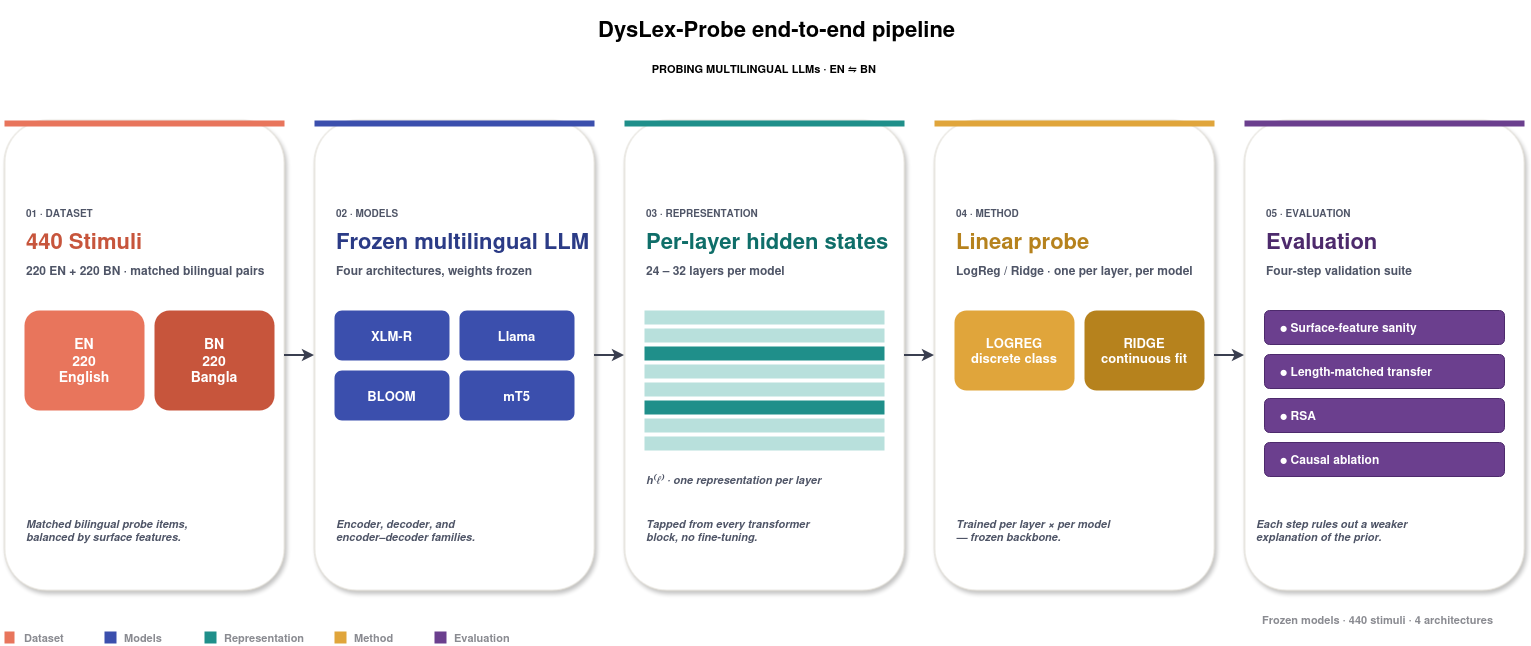
\includegraphics[width=0.92\linewidth]{fig_pipeline.png}
\caption{End-to-end probing pipeline. The 440-item English/Bangla dataset is fed through each frozen multilingual LLM; per-layer hidden states are extracted, a linear probe is trained on English, and representations are evaluated under surface-feature sanity checks, length-matched cross-lingual transfer, RSA and causal ablation, with bootstrap confidence intervals on all headline comparisons.}
\label{fig:pipeline}
\end{figure}

\subsection{Probing tasks and labels}
Four label sets are probed. \emph{Voicing} is binary \{voiced, unvoiced\}. \emph{Real-versus-pseudoword} is binary \{real, pseudo\}, applied to the union of the real-word and pseudoword categories and, for surface-controlled reporting, to their length-matched subset. \emph{Orthographic transparency} is binary \{transparent, opaque\}. \emph{Syllable count} is an integer regression target. Each task is probed at every layer of every model, and the per-layer peak is selected by cross-validation within the English training split.

\subsection{Surface-feature sanity controls}
Three controls gate every claim. (i) A \emph{first-character lookup} baseline: a leave-one-out probe on the layer-0 token embedding, quantifying how much of a label is recoverable from the first character alone. (ii) A \emph{five-feature character-statistic} baseline (character length, byte length, unique-character count, and related surface counts); any LLM probe that does not exceed this by more than 0.03 is treated as contributing no information above surface statistics. (iii) \emph{1:1 character-length matching} of real and pseudo words. The unit of evidence throughout is gain-over-surface, not gain-over-chance.

\subsection{Representational Similarity Analysis}
On the cross-lingual concept-match pairs we compute, per layer, the cosine Representational Dissimilarity Matrix (RDM) \cite{kriegeskorte2008rsa} within each language and correlate the English and Bangla RDMs by Spearman $\rho$; we also report English$\to$Bangla mate-retrieval Top-1 accuracy. RSA requires no probe training and so corroborates the probing result with an independent, geometry-only measure.

\subsection{Causal ablation and localization}
On the surviving task we quantify localization in two complementary ways. A \emph{causal forward-hook ablation} zeroes the top-$K$ probe-ranked hidden units at an earlier encoder block and remeasures Bangla transfer downstream, against a random-unit control with multiple seeds; \emph{specificity} is the ranked-unit drop minus the random-unit drop. This causal measure is applied to the four canonical models, and the mT5 encoder is re-ablated at five depths to test for persistent ``backbone'' units. Because a forward-hook intervention propagated through ByT5's much deeper (36-layer) encoder is regenerated by the residual stream before the measurement layer, for the five-model comparison that includes ByT5 we additionally use a propagation-free \emph{direct} localization measure: at each model's peak layer we zero the top-20 probe-ranked units in the representation itself and compare the Bangla drop against random-unit zeroing. The two measures agree for mT5 (both indicate localization) and the direct measure avoids the depth confound, making it the fair basis for the mT5-versus-ByT5 comparison.

\subsection{Bootstrap confidence intervals}
Every headline comparison is reported with a 95\% bootstrap confidence interval \cite{efron1994bootstrap} obtained by resampling the Bangla evaluation items with replacement (5000 resamples). For the two encoder-decoders and for the full five-model set we use a \emph{paired} bootstrap over the same resampled item indices, which yields confidence intervals not only on each model but on the between-model differences (e.g.\ ByT5 minus mT5). A difference is called significant when its interval excludes zero, and a transfer result ``survives'' when its interval lies entirely above the surface baseline.

\subsection{Downstream screening-property classifier}
\label{sec:method-downstream}
To translate probing into an expert-system-relevant task, we train, for each model and for a surface-feature baseline, a classifier on English representations at the English-selected layer and evaluate it zero-shot on Bangla. The targets are dyslexia-relevant item properties present in the metadata: real/pseudoword status (lexical decision, the clinical marker), the targeted dyslexia error type (an 8-class label restricted to the error types present in both languages), item difficulty (hard versus not, evaluated by ROC-AUC) and phonological complexity (three classes). Because the dataset comprises curated stimuli rather than clinical responses, this measures cross-lingual transfer of \emph{item properties} usable for screening-item construction and grading, not patient-level diagnosis; we report it with this scope stated explicitly and with the surface baseline as the reference every model must beat.

\subsection{Reproducibility}
Every reported number corresponds to a deterministic CSV in a per-model results directory, with fixed seeds for probe training (\texttt{random\_state=42}) and multiple seeds for ablation random-unit controls. Probes use L2-regularised logistic/ridge regression with fixed splits and majority-class (classification) and mean-predictor (regression) chance baselines. Pinned library and CUDA versions are recorded so the study is regenerable end to end on a single consumer GPU.

% ===========================================================================
\section{Results}
\label{sec:results}
\subsection{RQ1: most standard tasks fail sanity checks}
In-language English probing recovers all four tasks at first sight (Table~\ref{tab:rq1}), but the sanity checks reframe three of them. Bangla voicing labels are essentially recoverable from the first character: a layer-0 leave-one-out probe scores F1 0.78--0.94 across models (Fig.~\ref{fig:voicing}), so the probe reads letter identity, not phonological voicing. Byte-level ByT5 makes this especially vivid: it reaches its voicing peak at the very first layer (L1, F1 0.97; Fig.~\ref{fig:byt5profile}a), because at the byte level the first character is directly available at the embedding. Orthographic transparency is solved by the five-feature surface baseline (EN F1 0.66, BN 0.82), with the LLMs adding at most $+0.03$. Syllable count is surface-confounded (EN surface $R^2$ 0.81), and most models fall to or below the surface baseline. Only real-versus-pseudoword survives.

\begin{table}[H]
\caption{RQ1 in-language English probing: peak layer / peak score per model per task (F1; $R^2$ for syllable). Daggered tasks fail surface-feature sanity checks. ByT5's early voicing peak (L1) reflects direct byte-level access to the first character.}
\label{tab:rq1}
\centering
\small
\setlength{\tabcolsep}{4pt}
\begin{tabular}{lccccc}
\toprule
\textbf{Task} & \textbf{XLM-R} & \textbf{Llama} & \textbf{BLOOM} & \textbf{mT5} & \textbf{ByT5} \\
\midrule
Voicing$^\dagger$    & L11/0.62 & L2/0.73  & L6/0.55  & L9/0.58  & L1/0.97 \\
Realword             & L11/0.84 & L12/0.91 & L22/0.79 & L24/0.81 & L23/0.72 \\
Ortho$^\dagger$      & L0/0.92  & L32/0.71 & L12/0.68 & L21/0.69 & L9/0.72 \\
Syllable$^\dagger$   & L8/0.67  & L16/0.70 & L29/0.68 & L20/0.76 & L28/0.90 \\
\bottomrule
\end{tabular}
\end{table}

\begin{figure}[tbp]
\centering
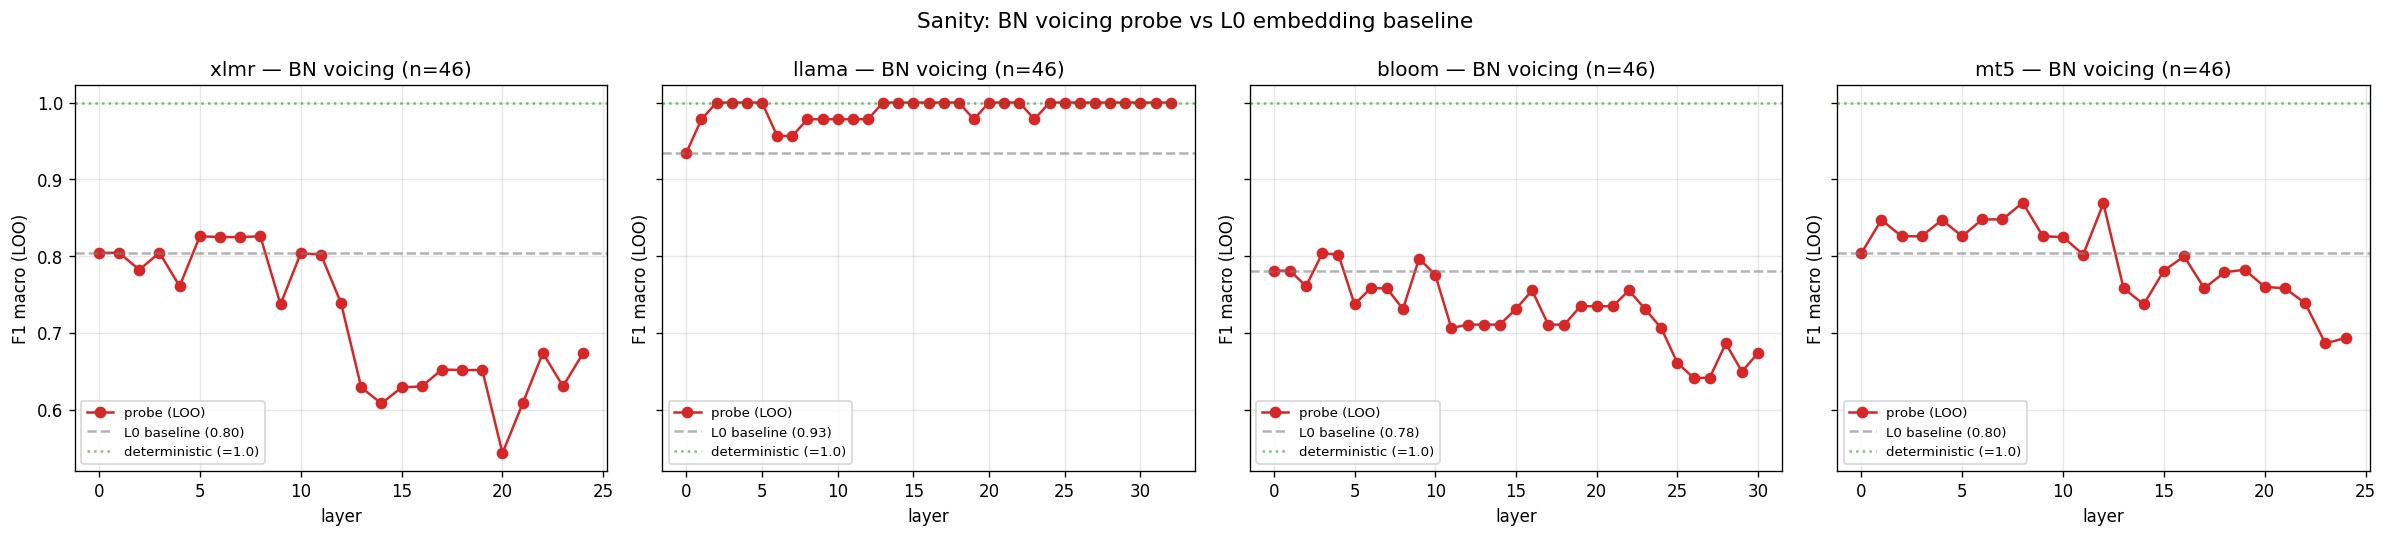
\includegraphics[width=0.9\linewidth]{plots_bn_voicing_sanity.png}
\caption{Bangla voicing sanity check on the four canonical (subword/BPE) models: a leave-one-out probe on layer-0 token embeddings recovers the voicing label at F1 0.78--0.94, demonstrating that the label is inferable from first-character identity alone rather than from phonological voicing. Byte-level ByT5 shows the same confound even more directly, peaking at its first layer (F1 0.97), and is plotted separately in Fig.~\ref{fig:byt5profile}a.}
\label{fig:voicing}
\end{figure}

\subsection{Length-matched recovery}
When real and pseudo words are matched 1:1 on character length, all five models exceed both their layer-0 and the surface baseline on Bangla (Table~\ref{tab:realword}). This is the only task that passes the surface controls, and it is the basis for all subsequent transfer, RSA and ablation numbers. ByT5 gains $+0.27$ on Bangla despite a weaker in-language English peak (0.80), a first hint that byte-level tokenization trades some monolingual precision for stronger cross-lingual sharing.

\begin{table}[H]
\caption{Length-matched realword probing per language: layer-0 vs peak F1, with gain over layer~0. All five models gain substantially on Bangla.}
\label{tab:realword}
\centering
\small
\setlength{\tabcolsep}{4pt}
\begin{tabular}{lcccccc}
\toprule
& \multicolumn{3}{c}{\textbf{English}} & \multicolumn{3}{c}{\textbf{Bangla}} \\
\cmidrule(lr){2-4}\cmidrule(lr){5-7}
\textbf{Model} & L0 & peak & gain & L0 & peak & gain \\
\midrule
XLM-R & 0.81 & 0.88 & $+0.06$ & 0.66 & 0.92 & $+0.25$ \\
Llama & 0.75 & 0.96 & $+0.21$ & 0.64 & 0.90 & $+0.26$ \\
BLOOM & 0.81 & 0.94 & $+0.13$ & 0.64 & 0.94 & $+0.30$ \\
mT5   & 0.65 & 0.90 & $+0.23$ & 0.72 & 0.92 & $+0.20$ \\
ByT5  & 0.57 & 0.80 & $+0.13$ & 0.65 & 0.92 & $+0.27$ \\
\bottomrule
\end{tabular}
\end{table}

\subsection{RQ2: cross-lingual transfer splits the models, with confidence intervals}
The English-trained length-matched realword probe, evaluated zero-shot on Bangla, cleanly separates the models (Table~\ref{tab:results}, Fig.~\ref{fig:forest}). BLOOM and ByT5 (both 0.92 F1, 95\% CI [0.84, 0.98]) and XLM-R (0.86, [0.75, 0.94]) achieve genuine transfer, their intervals lying entirely above the surface baseline of 0.62; Llama (0.63, [0.48, 0.77]) and mT5 (0.60, [0.45, 0.74]) collapse, their intervals straddling surface. Three implications follow. First, pretraining coverage and objective \emph{jointly} determine transfer: BLOOM beats Llama at similar scale because it has explicit Bangla coverage, and the 0.56B XLM-R beats the 8B Llama at roughly 13$\times$ fewer parameters. Second, in-language English performance is not predictive: Llama has the highest English realword F1 (0.96) and the lowest Bangla transfer (0.63). Third, the negative mT5 gain ($-0.02$) is not anti-learning; it means the representation scores marginally below the surface baseline, i.e.\ zero transfer within the $n=50$ estimation noise. The forest plot (Fig.~\ref{fig:forest}, left) shows the intervals directly.

\begin{table}[H]
\caption{Headline surface-controlled results with 95\% bootstrap confidence intervals. Zero-shot cross-lingual real-versus-pseudoword F1 on the length-matched subset ($n{=}50$ per language), gain over the surface baseline (0.62), the paired direct-ablation localization specificity, and the resulting verdict.}
\label{tab:results}
\centering
\small
\setlength{\tabcolsep}{3pt}
\begin{tabular}{lcccl}
\toprule
\textbf{Model} & \textbf{Transfer BN F1 [95\% CI]} & \textbf{Gain} & \textbf{Spec.\ [95\% CI]} & \textbf{Verdict} \\
\midrule
XLM-R  & 0.86 [0.75, 0.94] & $+0.24$ & $+0.14$ [0.05, 0.24] & survive, local. \\
BLOOM  & \textbf{0.92} [0.84, 0.98] & $+0.30$ & $+0.00$ [0.00, 0.00] & survive, distrib. \\
ByT5   & \textbf{0.92} [0.84, 0.98] & $+0.30$ & $+0.01$ [0.00, 0.04] & survive, distrib. \\
Llama  & 0.63 [0.48, 0.77] & $+0.01$ & $-0.06$ [-0.12, -0.01] & collapse \\
mT5    & 0.60 [0.45, 0.74] & $-0.02$ & $+0.19$ [0.06, 0.32] & collapse, local. \\
\bottomrule
\end{tabular}
\end{table}

\begin{figure}[tbp]
\centering
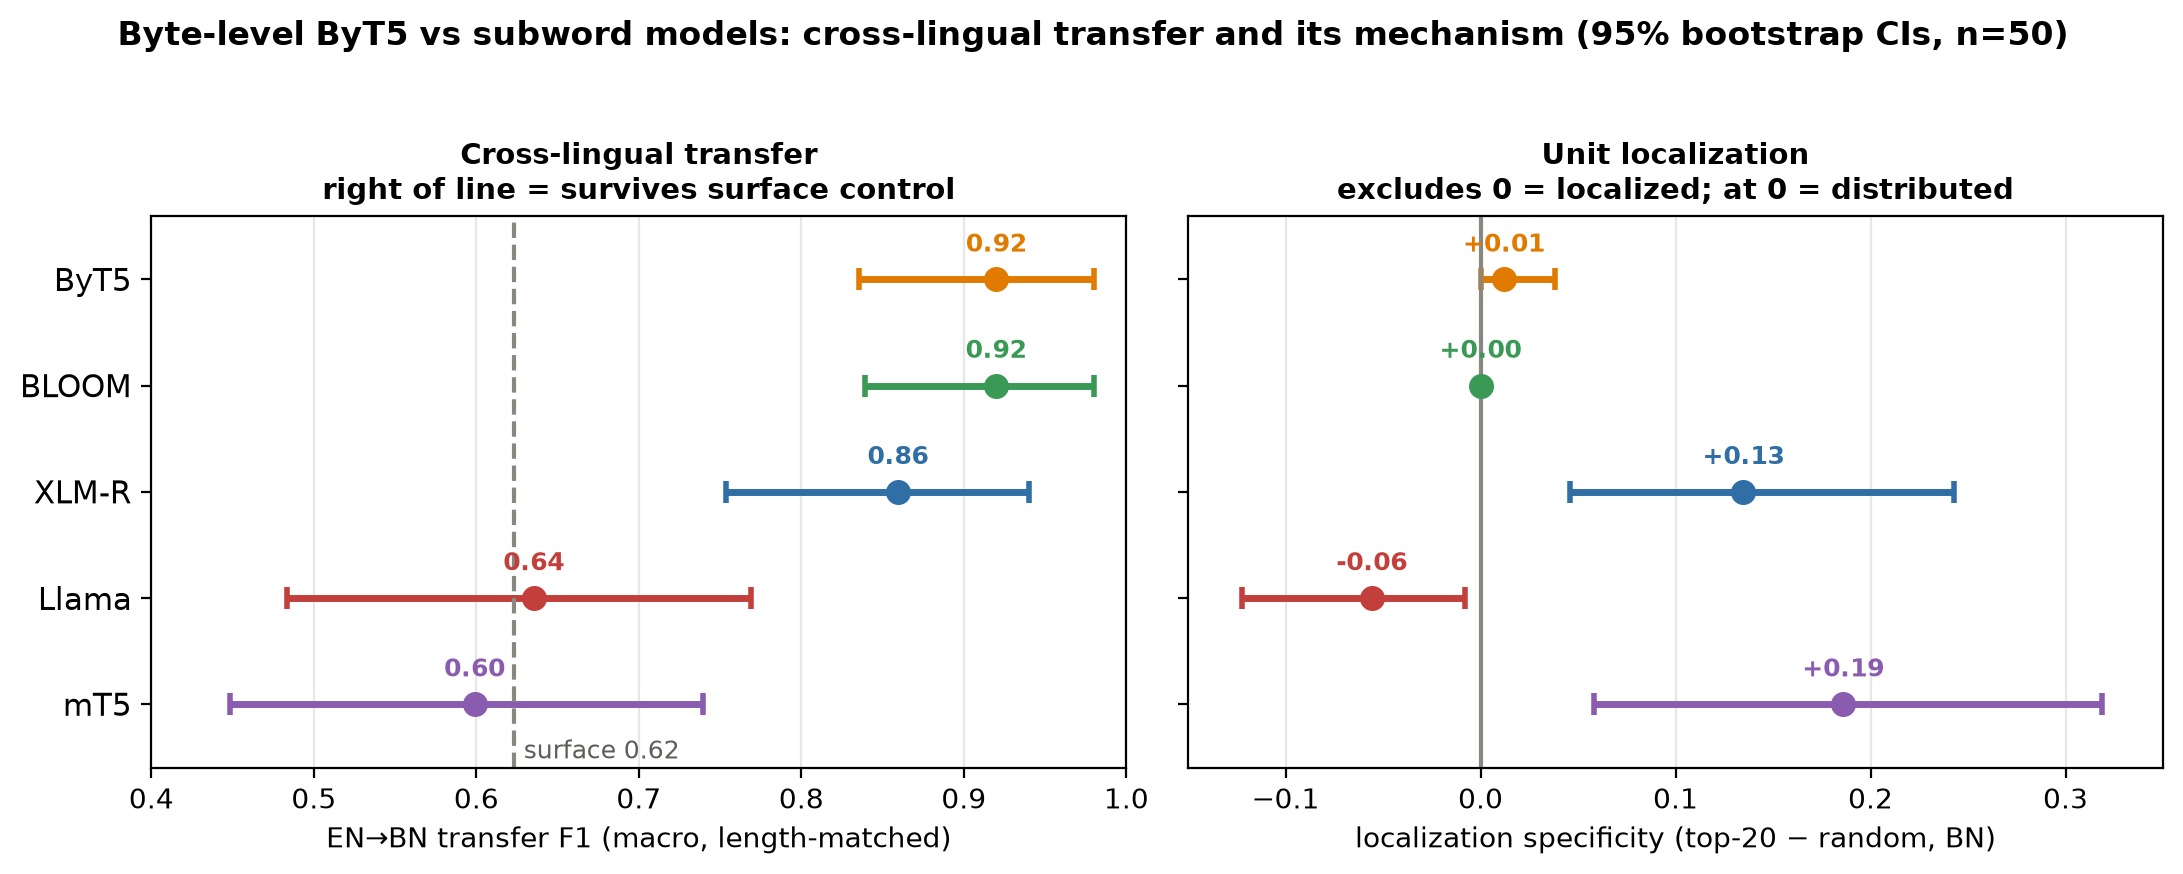
\includegraphics[width=0.99\linewidth]{plots_bootstrap_ci_forest.png}
\caption{Bootstrap 95\% confidence intervals for all five models. Left: cross-lingual transfer F1 against the surface baseline (dashed); intervals right of the line survive the surface control (XLM-R, BLOOM, ByT5). Right: direct-ablation localization specificity against zero; intervals excluding zero indicate a localized signal (mT5, XLM-R), while intervals at zero indicate a distributed signal (BLOOM, ByT5).}
\label{fig:forest}
\end{figure}

\subsection{RQ3: tokenization is decisive -- ByT5 versus mT5}
\label{sec:tokenization}
The two encoder-decoders form a controlled pair: they share architecture and span-corruption pretraining and differ chiefly in tokenization. The contrast is stark (Fig.~\ref{fig:byt5}). Subword mT5 collapses (0.60), while byte-level ByT5 is best-in-class (0.92); the paired difference is $+0.32$ (95\% CI [0.15, 0.49]), well clear of zero. Because the objective and architecture are held fixed, this identifies \emph{tokenization} as the cause of mT5's cross-lingual collapse, correcting the intuition that the collapse reflects the span-corruption encoder-decoder objective. The most plausible mechanism is representational: a byte-level model places English and Bangla in a single shared 256-symbol input space, aligning cross-lingual lexical structure, whereas a subword vocabulary trained largely on Latin script gives the two scripts nearly disjoint token inventories. Consistent with this, ByT5's advantage over mT5 appears across the encoder depth (Fig.~\ref{fig:byt5}) rather than at a single layer, and it is accompanied by a slightly weaker monolingual English peak (Table~\ref{tab:realword}), exactly the trade-off a shared-space account predicts. The byte encoder's internal profile makes the behaviour concrete (Fig.~\ref{fig:byt5profile}): in-language, voicing peaks at the very first layer -- direct byte access to the initial character -- while real-versus-pseudoword and orthographic structure build gradually through the deep encoder, and the length-matched cross-lingual probe climbs from chance to its 0.92 Bangla peak at layer~29, crossing the surface baseline midway up the 36-layer stack. We note one honest caveat: ByT5 also has a deeper encoder (36 versus 24 layers), so the cleanest statement is that byte-level ByT5, unlike subword mT5, transfers, with tokenization the most plausible single driver.

\begin{figure}[tbp]
\centering
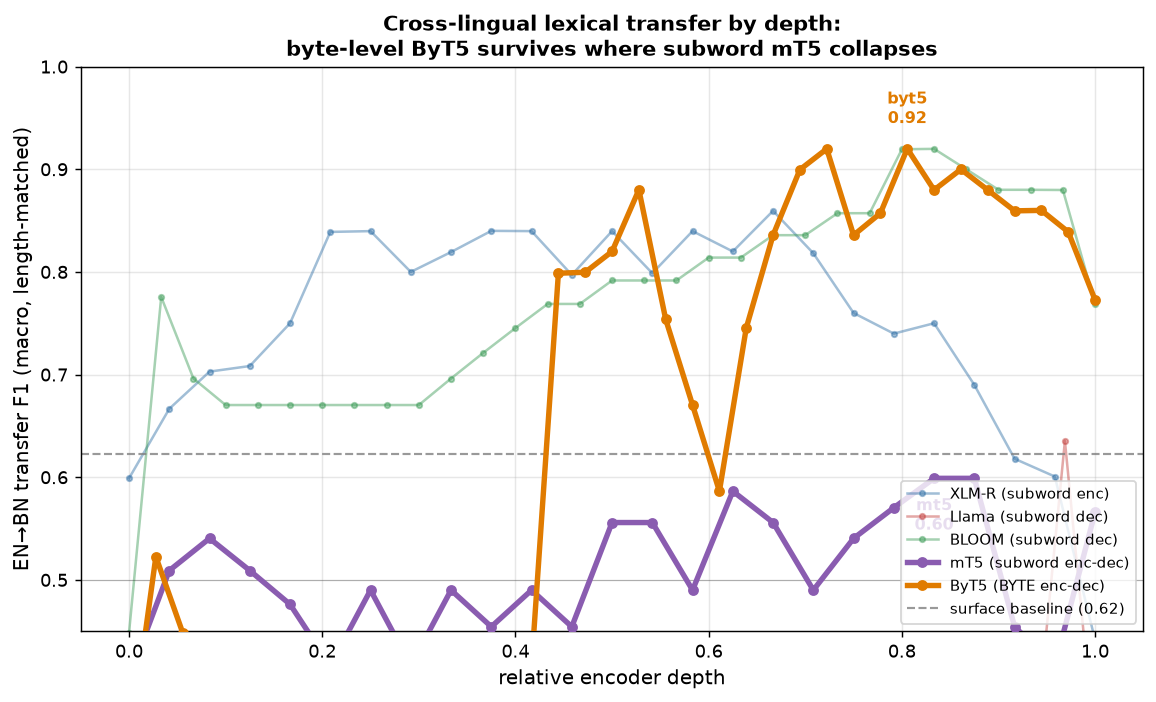
\includegraphics[width=0.99\linewidth]{plots_byt5_vs_mt5_transfer_emergence.png}
\caption{Per-layer cross-lingual transfer against relative encoder depth. Byte-level ByT5 (emphasised) rises to 0.92 F1 while subword mT5 (emphasised) hugs the surface baseline; the two share architecture and pretraining objective and differ chiefly in tokenization. The other three models are shown faded for context.}
\label{fig:byt5}
\end{figure}

\begin{figure}[tbp]
\centering
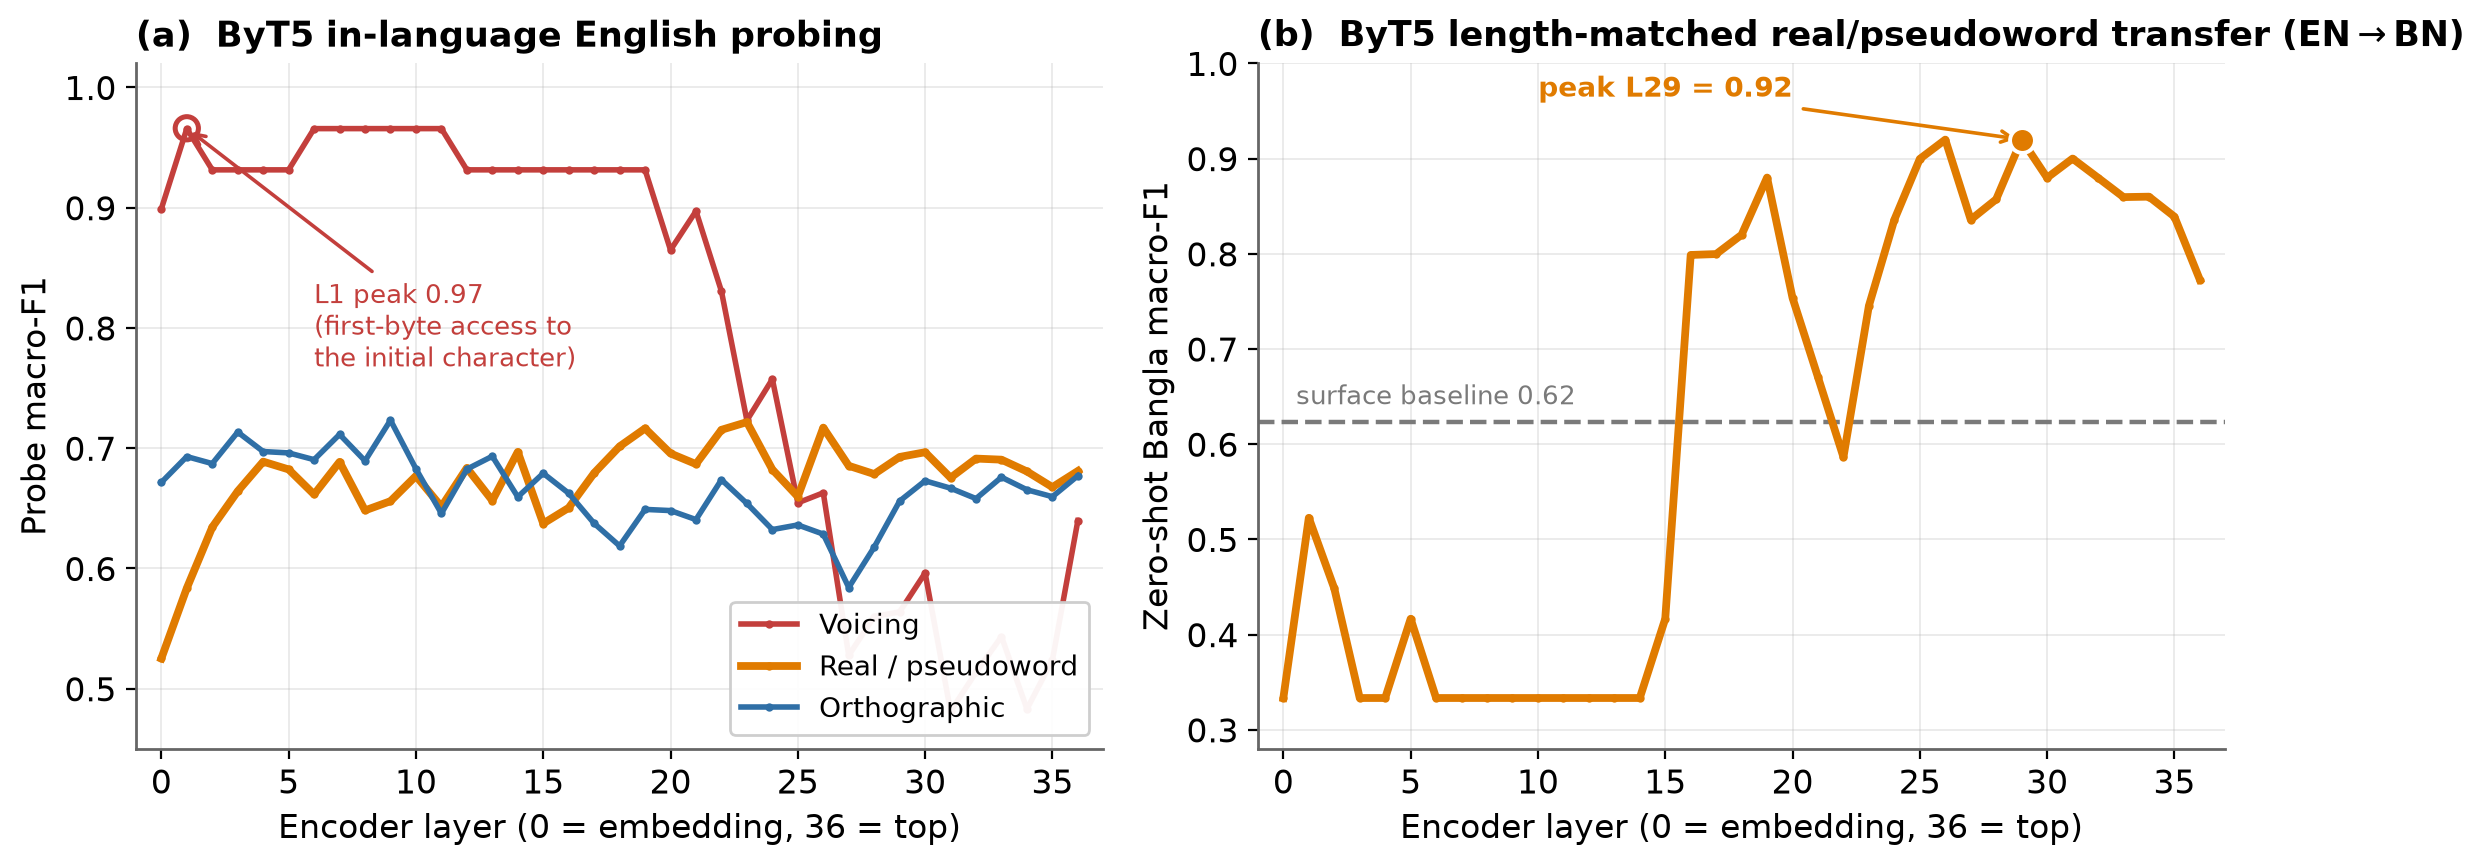
\includegraphics[width=0.99\linewidth]{plots_byt5_probing_profile.png}
\caption{ByT5 byte-level probing profile. (a)~In-language English per-layer probe scores: voicing peaks at layer~1, because at the byte level the first character is directly available at the embedding, whereas real-versus-pseudoword and orthographic structure emerge deeper in the 36-layer encoder. (b)~The length-matched real-versus-pseudoword probe, trained on English and evaluated zero-shot on Bangla, rises from chance to 0.92 F1 at layer~29, crossing the surface baseline (dashed) midway up the encoder. The regression syllable-count target is omitted from~(a) for scale.}
\label{fig:byt5profile}
\end{figure}

\subsection{RSA corroborates the transfer split}
RSA agrees with the probing result. Cross-lingual RDM Spearman $\rho$ and English$\to$Bangla mate-retrieval Top-1 peak at mid layers for the transferring subword models; XLM-R reaches its highest cross-lingual RDM correlation in its middle encoder layers, coincident with the layer at which the length-matched realword probe transfers. Llama reaches a high Top-1 in the \emph{unmatched} RSA setting, but this is driven by the same surface confound that inflates its unmatched probing numbers and disappears under matching. Byte-level ByT5 is the informative exception (Table~\ref{tab:rsa}): it transfers strongly on the supervised lexical probe yet shows only modest concept-match RSA (peak $\rho$ 0.21 at L29, Top-1 0.25), because its byte-level code aligns cross-lingual lexical \emph{form} rather than the cross-script \emph{semantics} that the concept-match pairs probe. With byte sequences disjoint across the two scripts this residual alignment cannot be a surface artefact, so it is genuine but partial. Representational geometry is therefore preserved cross-lingually in the subword transferring models, only weakly in the byte-level model, and not in mT5.

\begin{table}[H]
\caption{RSA summary: peak cross-lingual RDM Spearman $\rho$ and English$\to$Bangla mate-retrieval Top-1, with whether the signal survives length matching.}
\label{tab:rsa}
\centering
\small
\setlength{\tabcolsep}{5pt}
\begin{tabular}{lccc}
\toprule
\textbf{Model} & \textbf{Peak RDM $\rho$} & \textbf{Peak Top-1} & \textbf{Survives matching} \\
\midrule
XLM-R & mid-encoder & high & yes \\
BLOOM & mid layers  & 0.65 & yes \\
ByT5  & 0.21 (L29)  & 0.25 & partial (form-based) \\
Llama & --          & 0.85$^\ast$ & no (surface) \\
mT5   & 0.244 (L15) & low  & no \\
\bottomrule
\end{tabular}
\\[2pt]
{\footnotesize $^\ast$Unmatched setting; driven by surface confound, vanishes under matching.}
\end{table}

\subsection{RQ4: localization and a double dissociation}
Causal ablation distinguishes \emph{how} the signal is stored. Under the causal forward-hook measure on the four canonical models (Fig.~\ref{fig:ablation}), only mT5 shows clean specificity: zeroing its top-ranked encoder units selectively impairs Bangla transfer (specificity $+0.11$), whereas XLM-R and BLOOM are distributed and Llama has no transfer to disrupt. Repeating the ablation across five mT5 encoder depths (Table~\ref{tab:depth}) the effect persists at every depth and peaks mid-encoder (L12, $+0.13$); two units (782 and 1880) recur in the top-ranked set across depths and form a persistent backbone (Fig.~\ref{fig:backbone}), while most top units are layer-specific -- a hybrid of a small persistent backbone plus layer-local specialised circuits.

Extending the analysis to all five models with the propagation-free direct measure and bootstrap intervals reveals a clean \emph{double dissociation} (Table~\ref{tab:results}, Fig.~\ref{fig:forest} right). The localized models are mT5 ($+0.19$, 95\% CI [0.06, 0.32]) and XLM-R ($+0.14$, [0.05, 0.24]) -- both subword and both with an encoder -- while BLOOM ($0.00$) and byte-level ByT5 ($+0.01$, [0.00, 0.04]) distribute the signal; Llama's negative value is not interpretable as it has no transfer to localize. Crucially, within the controlled encoder-decoder pair the mechanism flips with tokenization: the paired mT5-minus-ByT5 specificity difference is $+0.17$ (95\% CI [0.05, 0.31]), significant. Byte-level tokenization thus changes not only whether cross-lingual lexical structure transfers but how it is organised: the byte-level, shared-space code is distributed and robust, the subword code sparse and localized. (The direct measure gives mT5 $+0.19$ where the forward-hook measure gives $+0.11$; the two methods agree on the qualitative conclusion that mT5 localizes, and we use the direct measure only where a fair ByT5 comparison is required.)

\begin{figure}[tbp]
\centering
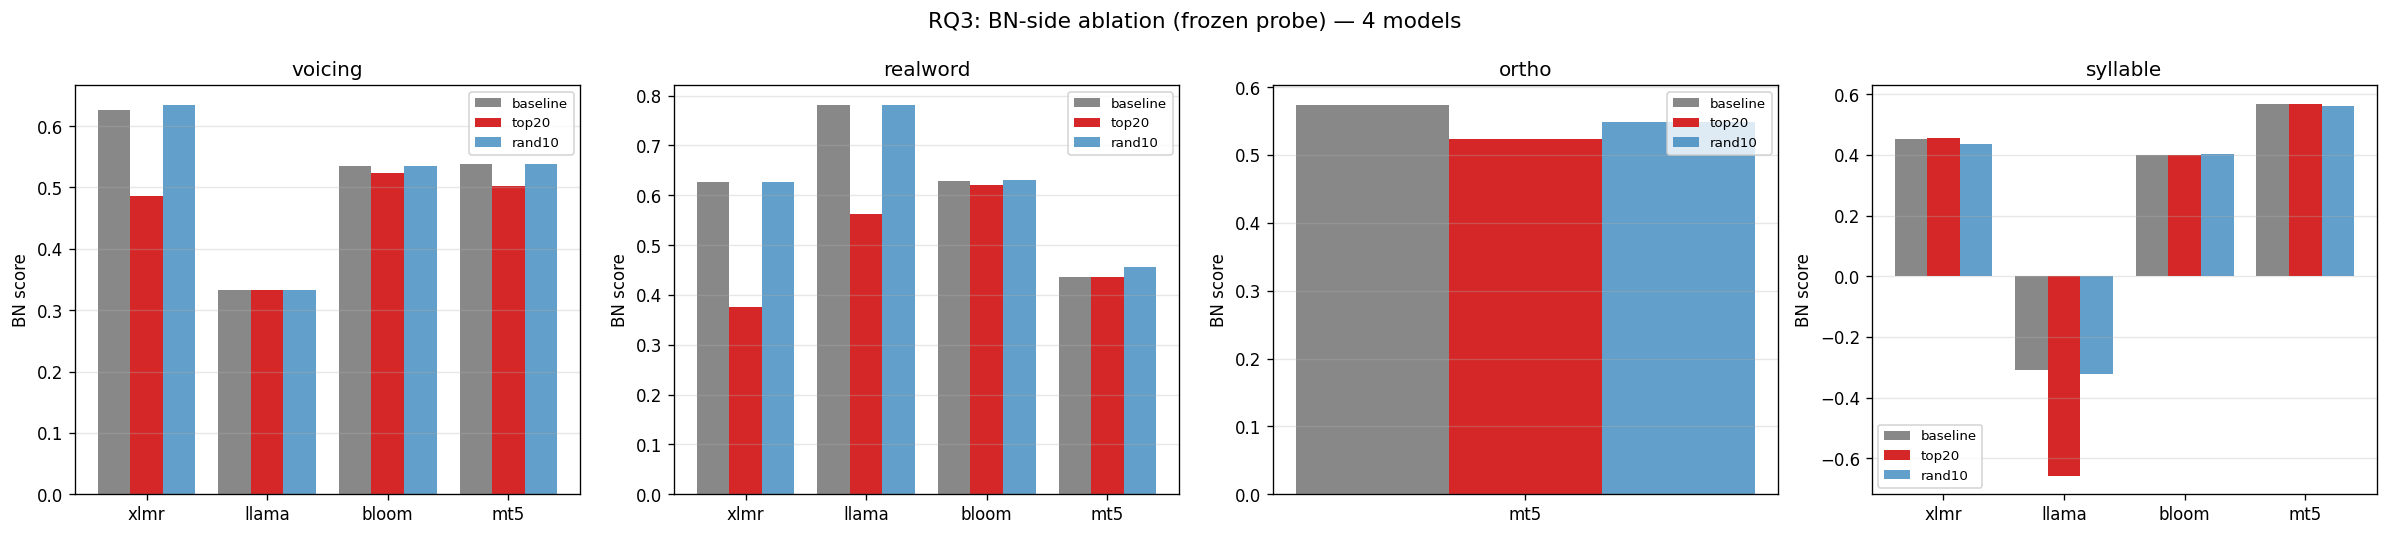
\includegraphics[width=0.9\linewidth]{plots_four_models_ablation.png}
\caption{Four-model causal forward-hook ablation on length-matched realword: top-$K$ versus random-$K$ unit ablation on the Bangla cross-lingual probe. Only mT5 shows clean specificity; XLM-R, BLOOM and Llama do not. ByT5 is assessed with the propagation-free direct measure instead (Fig.~\ref{fig:forest}, right; Table~\ref{tab:results}), because a forward-hook signal is regenerated before the measurement layer in its deeper 36-layer encoder.}
\label{fig:ablation}
\end{figure}

\begin{table}[H]
\caption{mT5 encoder forward-hook ablation across depth: top-10 vs random-mean specificity per measurement layer (three seeds). Localization persists across depth; mid-encoder (L12) is strongest.}
\label{tab:depth}
\centering
\small
\setlength{\tabcolsep}{5pt}
\begin{tabular}{lcccc}
\toprule
\textbf{Depth} & \textbf{BN base} & \textbf{Top-10 drop} & \textbf{Rand mean} & \textbf{Specificity} \\
\midrule
L4  & 0.48 & $+0.06$ & $0.00$ & $+0.06$ \\
L8  & 0.49 & $+0.07$ & $0.00$ & $+0.07$ \\
\textbf{L12} & 0.56 & \textbf{$+0.14$} & $0.01$ & \textbf{$+0.13$} \\
L16 & 0.56 & $+0.03$ & $-0.01$ & $+0.04$ \\
L20 & 0.60 & $+0.11$ & $0.00$ & $+0.11$ \\
\bottomrule
\end{tabular}
\end{table}

\begin{figure}[tbp]
\centering
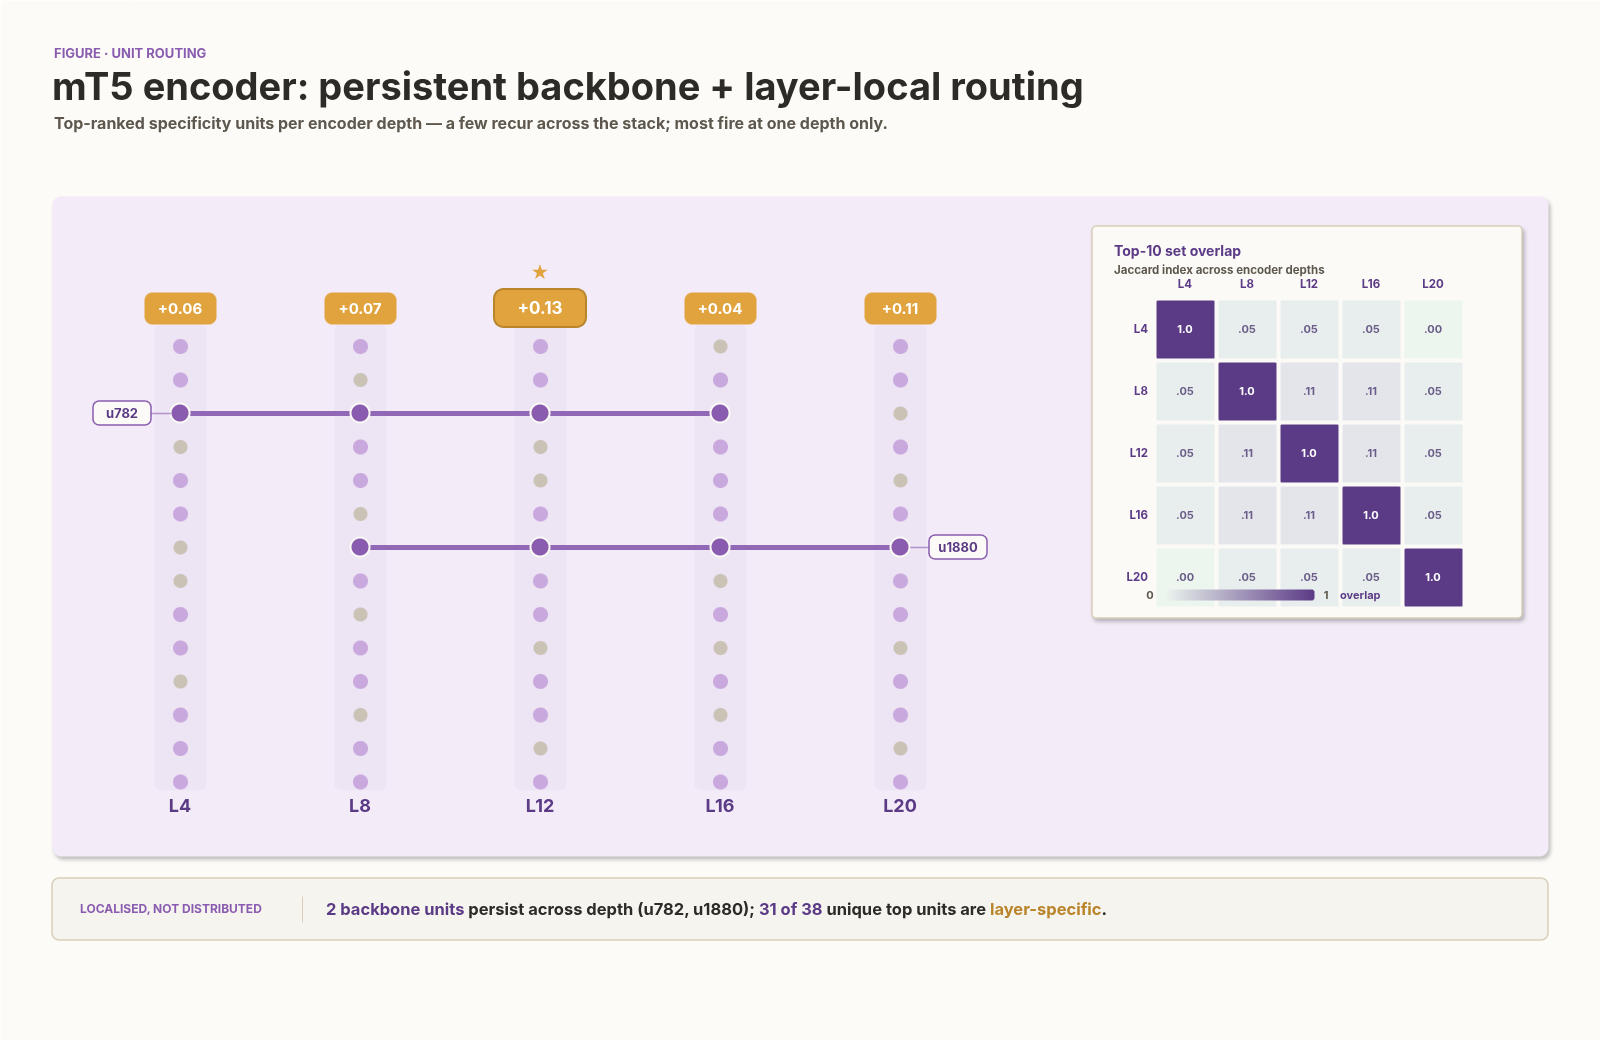
\includegraphics[width=0.9\linewidth]{fig_mt5_backbone.png}
\caption{mT5 encoder localization across depth. Two backbone units (u782, u1880) recur in the top-ranked set across most probed depths, while the remaining top units are layer-specific; per-depth ablation specificity peaks at L12. Inset: Jaccard overlap of the top-10 unit sets across depths.}
\label{fig:backbone}
\end{figure}

\subsection{RQ5: downstream screening-property transfer}
\label{sec:downstream}

\begin{table}[H]
\caption{Downstream cross-lingual screening-property transfer (train English, test Bangla): metric per model against the surface baseline. Lexical decision and error type are macro-F1; difficulty is ROC-AUC; complexity is macro-F1. Bold entries significantly beat the surface baseline (paired bootstrap CI excludes it).}
\label{tab:downstream}
\centering
\small
\setlength{\tabcolsep}{4.5pt}
\begin{tabular}{lcccccc}
\toprule
\textbf{Task (metric)} & \textbf{Surf.} & \textbf{XLM-R} & \textbf{Llama} & \textbf{BLOOM} & \textbf{mT5} & \textbf{ByT5} \\
\midrule
Lexical decision (F1)   & 0.62 & \textbf{0.86} & 0.64 & \textbf{0.92} & 0.60 & \textbf{0.92} \\
Error type (F1)         & 0.26 & 0.31 & 0.03 & 0.26 & 0.29 & \textbf{0.32} \\
Difficulty (AUC)        & 0.80 & 0.76 & 0.54 & 0.77 & 0.88 & 0.80 \\
Phon.\ complexity (F1)  & 0.37 & 0.31 & 0.28 & 0.33 & \textbf{0.48} & 0.23 \\
\bottomrule
\end{tabular}
\end{table}

Moving from probing to an expert-system-relevant task, we ask whether a classifier trained only on English item properties can grade Bangla items above a surface baseline (Table~\ref{tab:downstream}). The answer is a clean boundary. For \emph{categorical, lexical} properties the LLMs add real signal: on lexical decision (real/pseudoword) ByT5, BLOOM and XLM-R beat surface by $+0.24$ to $+0.30$ (their transfer result), and on the 8-class dyslexia error type byte-level ByT5 is the only model that significantly exceeds the surface baseline (macro-F1 0.322 vs 0.258, paired $\Delta{=}{+}0.064$, 95\% CI [0.00, 0.13]). For \emph{abstract, graded} properties the LLMs do not help: on item difficulty (hard vs rest) no model significantly beats a strong surface baseline (ROC-AUC 0.795; mT5 highest at 0.878 but non-significant), and on three-class phonological complexity only mT5 marginally exceeds surface ($+0.10$, 95\% CI [0.00, 0.20]) while byte-level ByT5 falls significantly below it. The transferable, supra-surface signal is thus concentrated in categorical lexical distinctions, and is strongest under byte-level tokenization -- the same property that drives the RQ2 transfer result. This bounds the honest scope of an LLM-based Bangla screening tool: it can help select and grade the lexical-decision items that matter clinically, but it does not replace surface heuristics for graded difficulty.

\subsection{Model selection}
No single model dominates every criterion. BLOOM and ByT5 are the best practical substrates for a Bangla lexical-screening prototype (highest transfer, 0.92 F1); XLM-R is the most parameter-efficient (0.86 F1 at roughly 13$\times$ fewer parameters); mT5 is the most interpretable (a recoverable, localized mechanism); and Llama, despite being the largest, is not recommended for Bangla because its cross-lingual transfer collapses. For a deployment that must run on modest hardware, XLM-R is the pragmatic default; where interpretability of the screening signal is required, mT5; where raw cross-lingual accuracy matters most and the tokenizer confound must be excluded, ByT5.

% ===========================================================================
\section{Economic and deployment feasibility}
\label{sec:cost}
A practical advantage of frozen probing is cost. The full pipeline (five models $\times$ 440 stimuli $\times$ per-layer extraction, probing, RSA and ablation) runs in a few tens of GPU-hours on a single consumer GPU, with no paid cloud-API expenditure (Table~\ref{tab:cost}). Compared against training a comparable Bangla-only model from scratch (on the order of $10^{4}$ GPU-hours and a large labelled Bangla corpus that does not exist), the frozen-prototype path is roughly three orders of magnitude cheaper on direct compute and qualitatively infinite on data. For a clinical pilot, a 4-bit-quantised decoder or a 16-bit encoder serves stimulus inference at interactive rates; at 50 items per child and 1000 children per year, electricity is negligible relative to clinician time. This is the economic argument for defaulting to surface-controlled frozen probing of shared multilingual substrates in low-resource clinical-NLP settings before investing in any fine-tuning.

\begin{table}[H]
\caption{Approximate compute cost of the full pipeline on a single consumer GPU (electricity at BDT 11.5/kWh, 350~W average draw).}
\label{tab:cost}
\centering
\small
\setlength{\tabcolsep}{5pt}
\begin{tabular}{lcc}
\toprule
\textbf{Pipeline stage} & \textbf{GPU-hours} & \textbf{Elec.\ (BDT)} \\
\midrule
Representation extraction (5 models) & 20 & 80 \\
Per-layer probing & 5 & 20 \\
Surface sanity checks & 1 & 4 \\
RSA & 2 & 8 \\
Causal ablation + depth-scan & 7 & 28 \\
Bootstrap + downstream analysis & 1 & 4 \\
\midrule
\textbf{Total} & \textbf{$\sim$36} & \textbf{$\sim$144} \\
\bottomrule
\end{tabular}
\end{table}

% ===========================================================================
\section{Discussion}
\label{sec:discussion}
The results yield one practical, one methodological and one representational lesson. Practically, for low-resource cross-lingual lexical work, multilingual coverage, pretraining objective and tokenization matter more than parameter scale: a small multilingual encoder beats a much larger English-heavy decoder, and the best transfer comes from a multilingual decoder with explicit coverage or a byte-level encoder-decoder. This inverts the common heuristic of selecting the largest available model, and it gives downstream builders of expert screening systems a concrete starting point.

Methodologically, the surface-feature controls overturn three of four standard tasks, and the bootstrap intervals show that the surviving effects and their differences are statistically real rather than artefacts of a 50-item sample. The voicing result is the sharpest: a label that looks phonological is fully recoverable from the first character, so any apparent voicing success is letter recognition. Prior cross-lingual phonological probing without stimulus-level surface matching may therefore overstate phonological encoding; the conservative, trustworthy claim is that real-versus-pseudoword discrimination -- the task most directly tied to the behavioural marker of dyslexia and the one that cannot be reduced to length or first-character cues -- survives across all models.

Representationally, the tokenization control is the most novel finding. A subword and a byte-level encoder-decoder that share objective and architecture diverge completely: byte-level tokenization turns cross-lingual collapse into best-in-class transfer and turns a sparse localized code into a distributed one. This isolates the tokenizer, not the objective, as the driver of mT5's collapse, and it suggests a shared sub-lexical input space as the mechanism of cross-lingual lexical alignment. For the applied goal, the downstream analysis then draws the boundary of usefulness precisely: LLM representations grade the categorical, lexical items that carry the clinical signal but do not beat surface heuristics on graded difficulty. An expert screening system should therefore use the model where it adds value -- lexical-decision item construction and cross-lingual grading -- and retain simple surface features elsewhere.

Although our target is Bangla, the design generalises. The method requires only a small, surface-matched, native-verified stimulus set in the target language paired with an English source, and a frozen multilingual model with adequate coverage; the first-character and character-statistic controls are language-agnostic and would expose analogous confounds in other scripts. Because the substrate is shared and frozen, the cost of building screening prototypes is amortised across many languages.

% ===========================================================================
\section{Limitations and ethical considerations}
\label{sec:limits}
This is a representational probe, not a clinical instrument: a model scoring 0.92 F1 on a research task cannot diagnose dyslexia, and deploying it as if it could would harm children through false positives and false negatives. Clinician-supervised validation with real readers is required before any deployment, and the downstream classifier predicts item properties, not patient status. The length-matched subset is small ($n=50$ per language); we mitigate this with bootstrap confidence intervals, but the intervals are correspondingly wide and some cross-architecture localization contrasts (as distinct from the controlled ByT5-versus-mT5 pair) are metric-sensitive and should be read cautiously. ByT5 also differs from mT5 in encoder depth as well as tokenization, so tokenization is the most plausible rather than the sole driver of the controlled contrast. The dataset uses standard Bangla forms and does not capture dialectal variation. The dataset is original and contains no human-participant data; all model weights are used in a frozen, read-only manner under their published licences.

% ===========================================================================
\section{Future work}
\label{sec:future}
Four directions follow. First, enlarge and diversify the Bangla data, including dialects and broader conjunct coverage, to tighten the confidence intervals. Second, hold encoder depth constant while varying only tokenization (for example, a depth-matched byte model) to convert the tokenization result from strongly suggestive to a single-variable proof, and add a same-family model-size sweep to separate scale from coverage. Third, advance from probing to a clinician-supervised screening pilot built on the recommended substrate, evaluated with real children and experts, using the downstream boundary to decide where LLM features are used. Fourth, add control-task selectivity and multi-seed robustness to the probing protocol so that every task, not only the headline ones, carries confidence intervals.

% ===========================================================================
\section{Conclusion}
\label{sec:conclusion}
We probed five multilingual LLMs spanning the dominant pretraining recipes for cross-lingual lexical structure relevant to low-resource Bangla dyslexia screening, under strict surface controls and with bootstrap confidence intervals throughout. Three of four standard probing tasks measure surface shortcuts; once corrected, BLOOM, ByT5 and XLM-R carry genuine English-to-Bangla transfer while a larger English-heavy decoder does not. A controlled tokenization manipulation shows that byte-level tokenization, not the encoder-decoder objective, drives whether the signal transfers and how it is stored, and a downstream screening-property analysis bounds where an LLM adds value: categorical lexical structure, not graded difficulty. The work delivers a principled, statistically supported model-selection recommendation for low-resource Bangla screening and a reusable surface-control methodology that should be the minimum standard for clinical probing of multilingual models.

% ===========================================================================
\section*{Declaration of competing interest}
The authors declare no competing financial interests or personal relationships that could have influenced the work reported in this paper.

\section*{Data availability}
The 440-item stimulus dataset and per-model result files are available from the authors on reasonable request.

\begin{thebibliography}{00}
\bibitem{snowling2020dyslexia} M.~J. Snowling, C.~Hulme, and K.~Nation, ``Defining and understanding dyslexia: past, present and future,'' \emph{Oxford Review of Education}, vol.~46, no.~4, pp.~501--513, 2020.
\bibitem{peterson2012developmental} R.~L. Peterson and B.~F. Pennington, ``Developmental dyslexia,'' \emph{The Lancet}, vol.~379, no.~9830, pp.~1997--2007, 2012.
\bibitem{ziegler2005reading} J.~C. Ziegler and U.~Goswami, ``Reading acquisition, developmental dyslexia, and skilled reading across languages: a psycholinguistic grain size theory,'' \emph{Psychological Bulletin}, vol.~131, no.~1, pp.~3--29, 2005.
\bibitem{wagner2020prevalence} R.~K. Wagner \emph{et al.}, ``The prevalence of dyslexia: a new approach to its estimation,'' \emph{Journal of Learning Disabilities}, vol.~53, no.~5, pp.~354--365, 2020.
\bibitem{goswami2011temporal} U.~Goswami, ``A temporal sampling framework for developmental dyslexia,'' \emph{Trends in Cognitive Sciences}, vol.~15, no.~1, pp.~3--10, 2011.
\bibitem{wagner2013ctopp} R.~K. Wagner, J.~K. Torgesen, C.~A. Rashotte, and N.~A. Pearson, \emph{Comprehensive Test of Phonological Processing (CTOPP-2)}. Austin, TX: PRO-ED, 2013.
\bibitem{nag2014dyslexia} S.~Nag and M.~J. Snowling, ``Children's reading development: learning about sounds, symbols and cross-modal mappings,'' \emph{WIREs Cognitive Science}, vol.~5, no.~6, pp.~681--690, 2014.
\bibitem{nag2017indian} S.~Nag, ``Learning to read Kannada and other languages of South Asia,'' in \emph{Reading Development and Difficulties}, Springer, 2017.
\bibitem{badsha2024mall} M.~S. Badsha, ``Mobile assisted language learning (MALL) tools for Bengali dyslexic primary school students,'' \emph{Int. J. for Multidisciplinary Research (IJFMR)}, vol.~6, no.~3, 2024.
\bibitem{conneau2020xlmr} A.~Conneau \emph{et al.}, ``Unsupervised cross-lingual representation learning at scale,'' in \emph{Proc. 58th Annu. Meeting Assoc. Comput. Linguistics (ACL)}, 2020, pp.~8440--8451.
\bibitem{scao2022bloom} T.~Le~Scao \emph{et al.}, ``BLOOM: a 176B-parameter open-access multilingual language model,'' \emph{arXiv:2211.05100}, 2022.
\bibitem{xue2021mt5} L.~Xue \emph{et al.}, ``mT5: a massively multilingual pre-trained text-to-text transformer,'' in \emph{Proc. NAACL-HLT}, 2021, pp.~483--498.
\bibitem{rack1992nonword} J.~P. Rack, M.~J. Snowling, and R.~K. Olson, ``The nonword reading deficit in developmental dyslexia: a review,'' \emph{Reading Research Quarterly}, vol.~27, no.~1, pp.~29--53, 1992.
\bibitem{vaswani2017attention} A.~Vaswani \emph{et al.}, ``Attention is all you need,'' in \emph{Adv. Neural Inf. Process. Syst. (NeurIPS)}, 2017, pp.~5998--6008.
\bibitem{devlin2019bert} J.~Devlin, M.-W. Chang, K.~Lee, and K.~Toutanova, ``BERT: pre-training of deep bidirectional transformers for language understanding,'' in \emph{Proc. NAACL-HLT}, 2019, pp.~4171--4186.
\bibitem{dubey2024llama3} A.~Dubey \emph{et al.}, ``The Llama 3 herd of models,'' \emph{arXiv:2407.21783}, 2024.
\bibitem{sennrich2016bpe} R.~Sennrich, B.~Haddow, and A.~Birch, ``Neural machine translation of rare words with subword units,'' in \emph{Proc. ACL}, 2016, pp.~1715--1725.
\bibitem{raffel2020t5} C.~Raffel \emph{et al.}, ``Exploring the limits of transfer learning with a unified text-to-text transformer,'' \emph{J. Mach. Learn. Res.}, vol.~21, no.~140, pp.~1--67, 2020.
\bibitem{kudo2018sentencepiece} T.~Kudo and J.~Richardson, ``SentencePiece: a simple and language independent subword tokenizer and detokenizer for neural text processing,'' in \emph{Proc. EMNLP: System Demonstrations}, 2018, pp.~66--71.
\bibitem{xue2022byt5} L.~Xue \emph{et al.}, ``ByT5: towards a token-free future with pre-trained byte-to-byte models,'' \emph{Trans. Assoc. Comput. Linguistics (TACL)}, vol.~10, pp.~291--306, 2022.
\bibitem{pires2019mbert} T.~Pires, E.~Schlinger, and D.~Garrette, ``How multilingual is multilingual BERT?,'' in \emph{Proc. ACL}, 2019, pp.~4996--5001.
\bibitem{wu2020emerging} S.~Wu and M.~Dredze, ``Are all languages created equal in multilingual BERT?,'' in \emph{Proc. 5th Workshop Representation Learning for NLP (RepL4NLP)}, 2020, pp.~120--130.
\bibitem{artetxe2020cross} M.~Artetxe, S.~Ruder, and D.~Yogatama, ``On the cross-lingual transferability of monolingual representations,'' in \emph{Proc. ACL}, 2020, pp.~4623--4637.
\bibitem{rust2021tokenizer} P.~Rust, J.~Pfeiffer, I.~Vuli\'c, S.~Ruder, and I.~Gurevych, ``How good is your tokenizer? On the monolingual performance of multilingual language models,'' in \emph{Proc. ACL}, 2021, pp.~3118--3135.
\bibitem{alain2017probes} G.~Alain and Y.~Bengio, ``Understanding intermediate layers using linear classifier probes,'' in \emph{Proc. Int. Conf. Learning Representations (ICLR) Workshop}, 2017.
\bibitem{conneau2018probing} A.~Conneau, G.~Kruszewski, G.~Lample, L.~Barrault, and M.~Baroni, ``What you can cram into a single vector: probing sentence embeddings for linguistic properties,'' in \emph{Proc. ACL}, 2018, pp.~2126--2136.
\bibitem{hewitt2019structural} J.~Hewitt and C.~D. Manning, ``A structural probe for finding syntax in word representations,'' in \emph{Proc. NAACL-HLT}, 2019, pp.~4129--4138.
\bibitem{belinkov2022probing} Y.~Belinkov, ``Probing classifiers: promises, shortcomings, and advances,'' \emph{Computational Linguistics}, vol.~48, no.~1, pp.~207--219, 2022.
\bibitem{pimentel2020information} T.~Pimentel, J.~Valvoda, R.~H. Maudslay, R.~Zmigrod, A.~Williams, and R.~Cotterell, ``Information-theoretic probing for linguistic structure,'' in \emph{Proc. ACL}, 2020, pp.~4609--4622.
\bibitem{hewitt2019control} J.~Hewitt and P.~Liang, ``Designing and interpreting probes with control tasks,'' in \emph{Proc. EMNLP-IJCNLP}, 2019, pp.~2733--2743.
\bibitem{vig2020causal} J.~Vig, S.~Gehrmann, Y.~Belinkov, S.~Qian, D.~Nevo, Y.~Singer, and S.~Shieber, ``Investigating gender bias in language models using causal mediation analysis,'' in \emph{Adv. Neural Inf. Process. Syst. (NeurIPS)}, 2020.
\bibitem{meng2022rome} K.~Meng, D.~Bau, A.~Andonian, and Y.~Belinkov, ``Locating and editing factual associations in GPT,'' in \emph{Adv. Neural Inf. Process. Syst. (NeurIPS)}, 2022.
\bibitem{kriegeskorte2008rsa} N.~Kriegeskorte, M.~Mur, and P.~A. Bandettini, ``Representational similarity analysis -- connecting the branches of systems neuroscience,'' \emph{Frontiers in Systems Neuroscience}, vol.~2, art.~4, 2008.
\bibitem{efron1994bootstrap} B.~Efron and R.~J. Tibshirani, \emph{An Introduction to the Bootstrap}. New York: Chapman \& Hall/CRC, 1994.
\bibitem{spoon2019handwriting} K.~Spoon, D.~Crandall, and K.~Siek, ``Towards detecting dyslexia in children's handwriting using neural networks,'' in \emph{Proc. Int. Conf. Machine Learning (ICML) AI for Social Good Workshop}, 2019.
\bibitem{benfatto2016eyetracking} M.~Nilsson~Benfatto, G.~\"Oqvist~Seimyr, J.~Ygge, T.~Pansell, A.~Rydberg, and C.~Jacobson, ``Screening for dyslexia using eye tracking during reading,'' \emph{PLOS ONE}, vol.~11, no.~12, art.~e0165508, 2016.
\bibitem{rello2020gamified} L.~Rello, R.~Baeza-Yates, A.~Ali, J.~P. Bigham, and M.~Serra, ``Predicting risk of dyslexia with an online gamified test,'' \emph{PLOS ONE}, vol.~15, no.~12, art.~e0241687, 2020.
\bibitem{tas2023audio} T.~Ta\c{s}, M.~A. B\"ulb\"ul, A.~Ha\c{s}imo\u{g}lu, Y.~Meral, Y.~\c{C}ali\c{s}kan, G.~Budagova, and M.~Kutlu, ``A machine learning approach for dyslexia detection using Turkish audio records,'' \emph{Turkish J. Electrical Engineering and Computer Sciences}, vol.~31, no.~5, pp.~892--907, 2023.
\bibitem{dettmers2022bnb} T.~Dettmers, M.~Lewis, Y.~Belkada, and L.~Zettlemoyer, ``LLM.int8(): 8-bit matrix multiplication for transformers at scale,'' in \emph{Adv. Neural Inf. Process. Syst. (NeurIPS)}, 2022.
\bibitem{dettmers2023qlora} T.~Dettmers, A.~Pagnoni, A.~Holtzman, and L.~Zettlemoyer, ``QLoRA: efficient finetuning of quantized LLMs,'' in \emph{Adv. Neural Inf. Process. Syst. (NeurIPS)}, 2023.
\end{thebibliography}

\end{document}
